\chapter{序論}
素粒子とは、物質を構成する最小単位の粒子のことである。
重力相互作用を除いた、強い相互作用、弱い相互作用、電磁相互作用の3つの相互作用を記述するための現代素粒子物理の基本的な枠組みを標準模型と呼ぶ。標準模型には、これまでにその存在が実験的に確かめられた17種類の素粒子が登場する。物質を構成する12種類のフェルミオン、相互作用を媒介する4種類のゲージボソン、他の粒子に質量を与えるヒッグス粒子である。~(図~\ref{fig:1-1})

\begin{figure}[h]
  \centering
  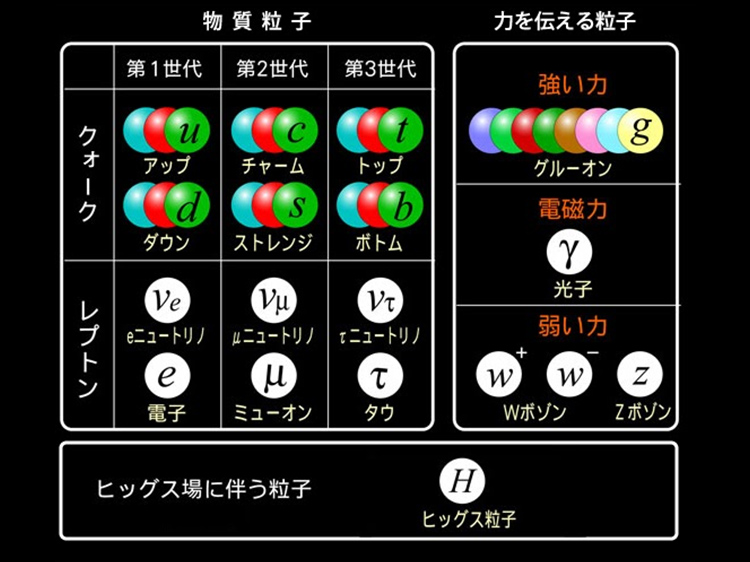
\includegraphics[clip, width=11cm]{fig/1/standardmodel_v2.jpg}
  \caption{標準模型を構成する17種類の素粒子。\cite{article:ATLAS_japan}}
  \label{fig:1-1}
\end{figure}

\newpage

標準模型は多くの実験結果を説明することのできる非常に優れた物理理論であるが、ヒッグスの階層性や宇宙・天体観測から存在がわかっている暗黒物質の正体など標準模型で説明できない問題が多く残っている。
そこで、これらの問題を解決するために世界中で様々な素粒子実験が行われている。

欧州原子核研究機構~(CERN)\cite{article:CERN}によって建設された~Large~Hadron~Collider~(LHC)\cite{article:LHC}を用いた素粒子実験である~ATLAS実験\cite{article:ATLAS}もその1つである。

ATLAS実験では、標準模型の精密測定に加えて超対称性粒子など標準模型を超えた物理現象の解明を目指し世界最高エネルギーでの高エネルギー素粒子実験が行われている。

LHC及びATLAS検出器は2018年から2022年までアップグレードが行われ、2022年7月から陽子陽子衝突の重心系エネルギー~($\sqrt{s}=13.6$)TeVで第三期運転~(Run-3)としてデータ取得が開始された。これまでほかの実験では到達できていないエネルギー領域において、新たな発見を目指す。